\documentclass[12pt]{article}
\usepackage{fullpage}
\usepackage{latexsym}
%\usepackage[utf8]{inputenc}
%\usepackage[T1]{fontenc}
\usepackage[danish,english]{babel}
\usepackage{amsmath}
\usepackage{amsfonts}
\usepackage{amssymb}
\usepackage{amsthm}
\usepackage{graphicx}
\usepackage{float}
\usepackage[ampersand]{easylist}
\usepackage{caption}
%%\usepackage{subcaption}
\usepackage{epstopdf}
\usepackage[format=hang,font=small]{caption} 	% Pretty captions
\usepackage{wrapfig} 
\usepackage{lscape}
\usepackage{subfig}
\usepackage{booktabs}
\usepackage{xcolor}
\usepackage{bbold}
\numberwithin{equation}{section}
\newcommand{\norm}[1]{\left\lVert #1 \right\rVert}
\newcommand{\avg}[1]{\left< #1 \right>}
\newcommand{\ket}[1]{\left| #1 \right\rangle}
\newcommand{\bra}[1]{\langle\left. #1 \right|}
\newcommand{\dprod}[2]{\langle #1 | #2 \rangle}
\newcommand{\Ohat}{\hat{\mathcal{O}}}
\newcommand{\fv}[1]{\mathbf{#1}}
\newcommand{\fp}{\mathbf{P}}
\newcommand{\pdif}[1]{\frac{\partial}{\partial #1}}
\newcommand{\rdif}[1]{\frac{d}{d #1}}
\newcommand{\cop}{c_{\uparrow}^{\phantom{\dagger}}}
\newcommand{\copd}{c_\uparrow^{\dagger}}
\newcommand{\cdown}{c_{\downarrow}^{\phantom{\dagger}}}
\newcommand{\cdownd}{c_\downarrow^\dagger}
\newcommand{\rref}[1]{(\ref{#1})}
\renewcommand{\v}[1]{\ensuremath{\mathbf{#1}}} % for vectors
\newcommand{\gv}[1]{\ensuremath{\mbox{\boldmath$ #1 $}}} % for vectors of Greek letter
\newcommand{\dint}[1]{\, \mathrm{d }#1}
\newcommand{\dintc}[1]{\mathrm{d} #1 \,} % For beautiful integration variable declaration such as dx
\newcommand{\sgn}{\mathrm{sgn}}
\newcommand{\matr}[1]{\underline{\underline{#1}}}
\newcommand{\A}{\mathcal{A}}
\usepackage{ulem}
\begin{document}

\section{Introduction}
This is a quick and dirty introduction to recurrent neural networks (RNNs) written mainly for my own sake.

RNNs are functions applied to sequences that output other sequences; typically (always?) the output is the predicted continuation of the input sequence. RNNs have been used for natural language processing and music generation. 

RNNs consist of a NN applied to each element in the input sequence where the NN also has inter-element connections. The same network is applied to each element, hence the name recurrent. This is not essential but at least drastically reduces the number of parameters to learn; it also solves the hard problem of how to define (not to mention train!) a potentially infinite set of NNs. A schematic of a RNN is show in the figure. 


\begin{figure}[H]
\centering
\includegraphics[width=0.4\textwidth]{RNNBasicUnit.pdf}
\caption{The basis neural net unit of a RNN.}
\end{figure}



\begin{figure}[H]
\centering
\includegraphics[width=0.4\textwidth]{RNNFull.pdf}
\caption{The RNN applied to a sequence of length 4.}
\end{figure}

Each step, numbered by \(t\), in the sequence has an input variable, \(x_t\) (indicated by the red circles on the left side), a hidden state pre-activation \(a_t\) (blue cicles on the left of the vertical line), a hidden state post-activation \(s_t\) (blue circles on the right of the vertical line), an output state pre-activation, \(p_t\) (blue circle on the right) and an output state post-activation \(o_t\) (red circle on the right). For our purposes the output \(o_t\) is interpreted as probabilities that the RNN assigns to the next element of the sequence, i.e. at step \(t+1\). The diagrams above are intended to illustrate that these numbers are calculated as
\begin{align}
a_t &= Ux_t + Ws_{t-1},\\
s_t &= \mathcal{A}(a_t), \\
p_t &= Vs_t, \\
o_t &= \mathcal{O}(p_t).
\end{align}
Here \(\mathcal{A}, \mathcal{O}\) are the activation and output activation functions, e.g. \(\tanh(x)\) and "softmax" for word processing RNNs. For the first element of the sequence one must choose an initialization of \(s_{-1}\), e.g. \(s_{-1} = 0\). We may only be interested in the output of the last element of the RNN, e.g. when we try to predict or generate the next word in a sentence or the next musical note. 

\section{Training of a RNN}
As with regular NNs training relies on formulas for the gradients calculated using the chain rule. In the case of RNNs the expressions are slightly more complicated because the same matrix appears in several places. E.g. \(a_t\) depends on \(U\) both through \(Ux_t\) and \(Ws_{t-1}\). We assume that the error can be written as
\begin{align}
E = \sum_t E_t,
\end{align}
which is not very restrictive.

Let us calculate the gradients \(\frac{\partial E_t}{\partial V}, \frac{\partial E_t}{\partial W}, \frac{\partial E_t}{\partial U}\). Since \(E_t\) depends only on the output of the RNN (and the target output but that is obviously independent of the parameters of the network) we can write
\begin{align}
\frac{\partial E_t}{\partial V} = \frac{\partial E_t}{\partial p_t} \frac{\partial p_t}{\partial V}.
\end{align}
Note that \(p_t\) is a vector and \(V\) is a matrix; if we write the above equation with indices we have
\begin{align}
\frac{\partial E_t}{\partial V_{ij}} =\sum_k \frac{\partial E_t}{\partial (p_t)_k} \frac{\partial (p_t)_k}{\partial V_{ij}}.
\end{align}
But let us just view \(\frac{\partial E_t}{\partial p_t}\) as a covariant/column vector and \(\frac{\partial p_t}{\partial V_{ij}}\) as a contravariant/column vector. Now, assuming we use the canonical link we have
\begin{align}
\frac{\partial E_t}{\partial p_t} = o_t - t_t,
\end{align}
where \(t_t\) is the target vector. Finally (for this gradient)
\begin{align}
\frac{\partial p_t}{\partial V} = \frac{\partial Vs_t}{\partial V} = s_t + V \frac{\partial s_t}{\partial V} = s_t + 0 = s_t. 
\end{align}
I have written every step explicitly to emphasize that the expression is only simple because \(s_t\) does not depend on \(V\):
\begin{align}
\frac{\partial E_t}{\partial V} = (o_t - t_t)\otimes s_t^T.
\end{align}
Here I have also emphasized that we end up with a matrix:
\begin{align}
\frac{\partial }{\partial A}x^TAy = \frac{\partial }{\partial A} \mathrm{Tr}Ayx^T = xy^T.
\end{align}

Next up:
\begin{align}
\label{start}
\frac{\partial E_t}{\partial W} &= \frac{\partial E_t}{\partial p_t} \frac{\partial p_t}{\partial W} = \frac{\partial E_t}{\partial p_t} \frac{\partial p_t}{\partial s_t} \frac{\partial s_t}{\partial W} \\
&= \frac{\partial E_t}{\partial p_t} \frac{\partial p_t}{\partial s_t} \frac{\partial s_t}{\partial a_t} \frac{\partial a_t}{\partial W} = \frac{\partial E_t}{\partial p_t} \frac{\partial p_t}{\partial s_t} \frac{\partial s_t}{\partial a_t} \frac{\partial(Ux_t+ Ws_{t-1})}{\partial W} \nonumber \\
&= \frac{\partial E_t}{\partial p_t} \frac{\partial p_t}{\partial s_t} \frac{\partial s_t}{\partial a_t} \left(s_{t-1} + W \frac{\partial s_{t-1}}{\partial W} \right). 
\end{align}
The form of the equation is now similar to the first line eq. \rref{start} (which is why it got its own label). To calculate the last factor we use the structure we already uncovered:
\begin{align}
\frac{\partial s_t}{\partial W} =  \frac{\partial s_t}{\partial a_t} \left(s_{t-1} + W \frac{\partial s_{t-1}}{\partial W} \right).
\end{align}
Applying this formula until we reach the first layer \(t=0\) allows us to calculate the full gradient \(\partial_W E_t\). Just so we all agree on the matrix structure we are working with here, let's state it explicitly: \(\frac{\partial s_t}{\partial a_t}\) is a matrix with entries
\begin{align}
\left( \frac{\partial s_t}{\partial a_t}\right)_{ij} = \frac{\partial (s_t)_i}{\partial (a_t)_j},
\end{align}
\(s_{t-1}, \frac{\partial s_{t-1}}{\partial W}\) are vectors.

Next in line:
\begin{align}
\frac{\partial E_t}{\partial U} &= \frac{\partial E_t}{\partial p_t} \frac{\partial p_t}{\partial s_t} \frac{\partial s_t}{\partial a_t} \frac{ \partial (Ux_t + Ws_{t-1})}{\partial U} = \frac{\partial E_t}{\partial p_t} \frac{\partial p_t}{\partial s_t} \frac{\partial s_t}{\partial a_t} \left( x_t + W \frac{\partial s_{t-1}}{\partial U}\right) 
\end{align}
Here the key formula is
\begin{align}
\frac{\partial s_{t}}{\partial U} = \frac{\partial s_t}{\partial a_t}\left(x_t + W \frac{\partial s_{t-1}}{\partial U}\right).
\end{align}


\section{LSTMs}
There are certain problems with regular RNNs. Gradients tend to go to zero as we move back along the sequence. This means that during training the output at \(T\) is not very sensitive to the input at \(t\ll T\). Obviously this is very bad for text generators or for musical nets that want to do more than just meander through a scale. I won't go into detail on the "vanishing gradient" problem, but take a look at wildml.com if you are interested.

Long-Short-term memory [neural networks] (LSTMs) combat this problem. LSTMs calculate the hidden state in a different way that intuitively allows information to more easily propagate from step to step. We introduce a "memory" at each step which is influenced by the input at the current step, the memory at the previous step as well as the hidden state at the previous step. Concretely the hidden state, \(s_t\) is now calculate by
\begin{align}
i_t &= \sigma(U^ix_t + W^is_{t-1}), \\
f_t &= \sigma(U^fx_t + W^f s_{t-1}), \\
o_t &= \sigma(U^o x_t + W^o s_{t-1}), \\
g_t &= \mathcal{A}(U^g x_t + W^gs_{t-1}), \\
c_t &= c_{t-1} \circ f_t + g_t \circ i_t, \\
s_t &= \mathcal{A}(c_t) \circ o_t,\\
y_t &= \mathcal{O}(Vs_t).
\end{align}
We have used \(\circ\) to indicate element-wise multiplication, \(\sigma(x) = \frac{1}{1+\exp(-x)}\) is the sigmoid function. We have also redefined what \(o\) means; this is just to match the notation on wildml.com. The output is now denoted by \(y_t\). It is quite complicated and can be illustrated like in the figure below.

\begin{figure}[H]
\centering
\includegraphics[width=0.8\textwidth]{LSTMBasicUnit.pdf}
\caption{}
\end{figure}

The derivate with respect to \(V\) is easy so let's skip that.

To calculate the other gradients let me introduce some new variables.
\begin{align}
d_t &= \mathcal{A}(c_t), \\
a_t &= U^gx_t + W^g s_{t-1}, \\
u_t &= U^o x_t + W^o s_{t-1}
\end{align}

\begin{align}
\frac{\partial E_t}{\partial W^o} &= \frac{\partial E_t}{\partial p_t}\frac{\partial p_t}{\partial W^o} = \frac{\partial E_t}{\partial p_t} \frac{\partial p_t}{\partial s_t}\frac{\partial s_t}{\partial W^o} \nonumber\\
&= \frac{\partial E_t}{\partial p_t} \frac{\partial p_t}{\partial s_t}\frac{\partial (d_t \circ o_t)}{\partial W^o} \nonumber \\
&= \frac{\partial E_t}{\partial p_t} \frac{\partial p_t}{\partial s_t}\left(\frac{\partial d_t }{\partial W^o}\circ o_t + d_t \circ \frac{\partial o_t}{\partial W^o}\right) \nonumber \\
&= \frac{\partial E_t}{\partial p_t} \frac{\partial p_t}{\partial s_t}\left(\frac{\partial d_t}{\partial W^o}\circ o_t + d_t \circ \frac{\partial o_t}{\partial W^o}\right) \nonumber \\
&= \frac{\partial E_t}{\partial p_t} \frac{\partial p_t}{\partial s_t}\left( \frac{\partial d_t}{\partial W^o}\circ o_t + d_t \circ \frac{\partial o_t}{\partial u_t}\frac{\partial u_t}{\partial s_{t-1}}\frac{\partial s_{t-1}}{\partial W^o}\right).
\end{align}






\end{document}